\documentclass[a4paper,11pt]{article}
\usepackage[utf8]{inputenc}
\usepackage{graphicx}
\usepackage[english]{babel}
\usepackage[vmargin=3.5cm, top=2cm]{geometry}
\usepackage[linktocpage=true]{hyperref}
\usepackage{enumitem}
\usepackage{longtable}
\usepackage{pdfpages}
\usepackage{float}
\usepackage{hyperref}
\usepackage[section]{placeins}
\hypersetup{
   colorlinks,
   citecolor=black,
   filecolor=black,
   linkcolor=black,
   urlcolor=black
}

\begin{document}

\begin{titlepage}

\centering \parindent=0pt
\newcommand{\HRule}{\rule{\textwidth}{1mm}}
\vspace*{\stretch{1}} \HRule\\[1cm]\Huge\bfseries
Data Mining Report\\[0.7cm]
\HRule\\[4cm]  
\large by 
\\ Mikkel Stolborg
\\ Hlynur Örn Haraldsson
\vspace*{\stretch{2}} \normalsize %
\begin{flushleft}
IT University of Copenhagen \\
MDMI, S2015\\
Anders Hartvig Hartzen\\
Hajira Jabeen\\
Héctor Pérez Martínez\\
Sebastian Risi\\
Noor Shaker\\
\today \end{flushleft}
\end{titlepage}

\tableofcontents
\pagebreak
\section{Introduction}
\subsection{Data selection}

\subsection{Research question}
Our primary question which we want answered was:\\
\textit{"Which attributes contributes mostly to the survival rate of a passenger on the Titanic}\\
Here we wished to figure out what set of parameters would ensure the highest rate of survival on the Titanic. We would use classification through a classification tree to figure out which set gives the highest percentage of survival.

The secondary question arose when looking at clusters of the data.\\
\textit{"Which societal data can be found in clusters of the titanic data"}\\
Looking at the data, we decide to try clustering to see if there was an emergent pattern. It would be interesting to see if the were a relation between wealth and number of children and the like. 
\subsection{Tools for data mining}
We choose to use the free tool called Orange\cite{orange}. This tool allowed to quickly manipulate the data, such that we could extract the interesting elements. 
In the tool you manipulate the data by clicking and drawing connections between data elements and processing methods. Before explaining further, we have included the map of the process used for our data set in the orange framework, see figure \ref{OrangeMap}.

\begin{figure}[h]
	\centering
	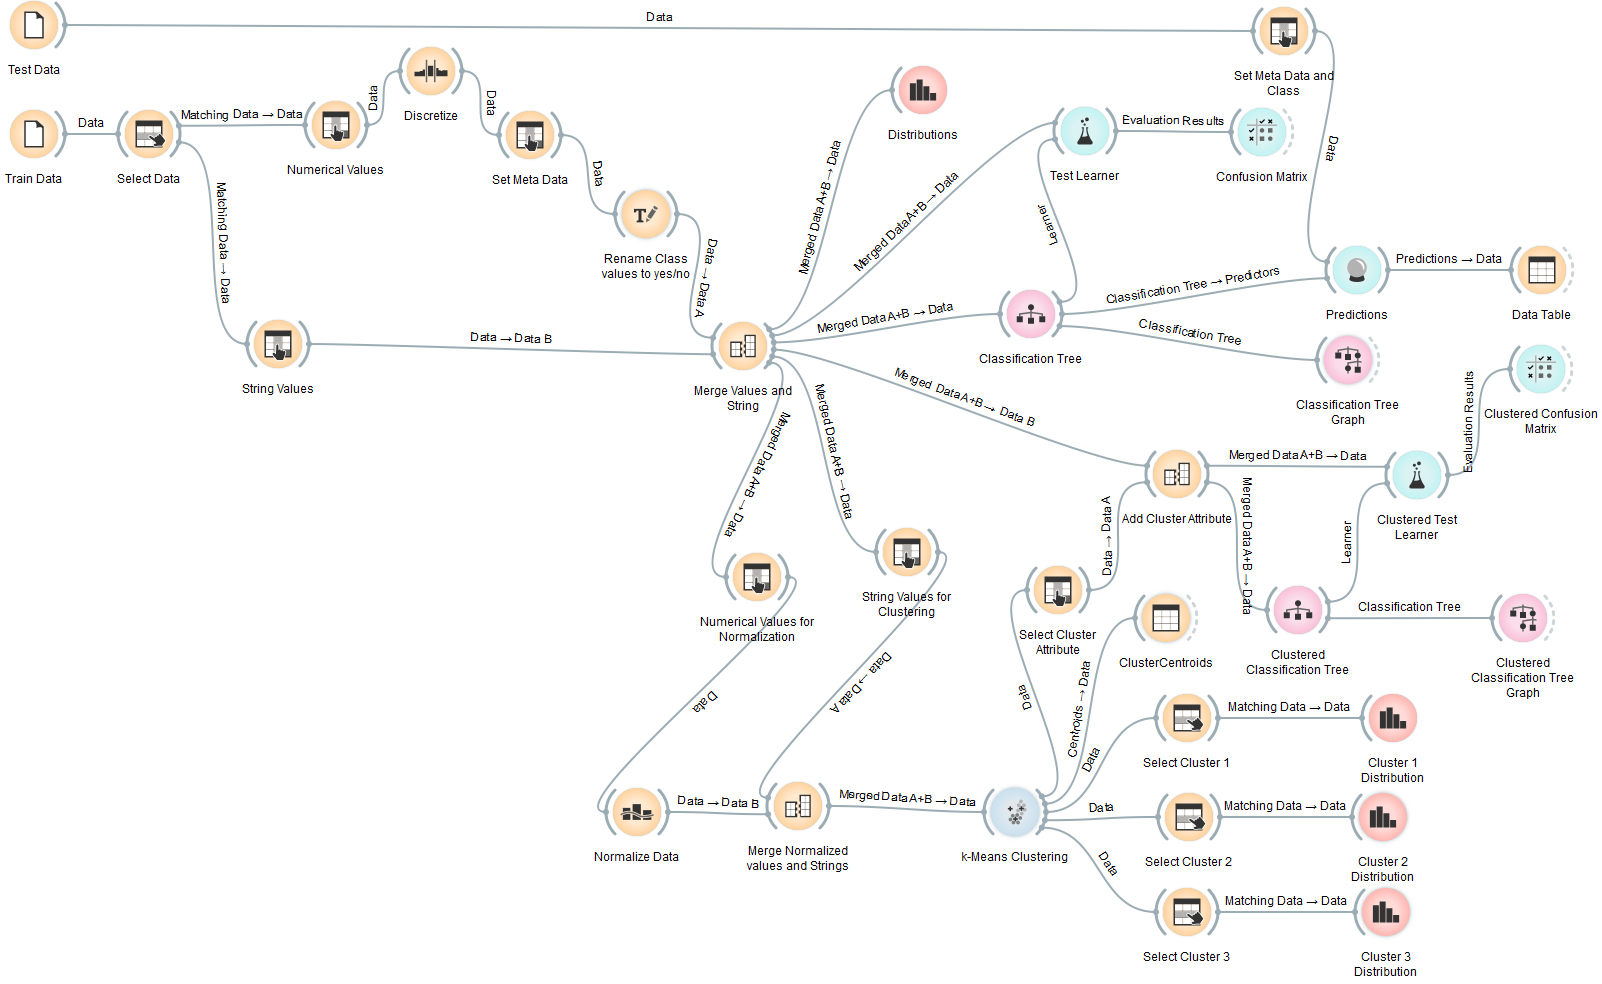
\includegraphics[scale=0.35]{orangeMap}
	\caption{The map of the methods and processes used on the data.}
	\label{OrangeMap}
\end{figure}


\section{Data mining}
\subsection{Preprocessing}
\subsection{Classification tree}
\subsubsection{Cross Validation}
\subsection{K-means Clustering}
\subsubsection{Data validation}

\section{Conclusion}
\subsection{Societal impact}




\appendix
\begin{thebibliography}{9}

\bibitem{orange}
  \emph{Orange Data Mining},
  http://orange.biolab.si/,
  13-05-15
\end{thebibliography}

\end{document}


